\documentclass[10pt,a4paper]{article}
\usepackage[T1]{fontenc}
\usepackage{lmodern,textcomp}
\usepackage[margin=2.4cm]{geometry}
\usepackage{amsmath,amssymb,amsthm}
\usepackage{graphicx,booktabs,array,float}
\usepackage[hidelinks]{hyperref}
\usepackage{microtype}
\setlength{\parskip}{3pt}
\newtheorem{proposition}{Proposition}
\newtheorem{definition}{Definition}
\renewcommand{\arraystretch}{1.1}
\begin{document}
\title{\bfseries Media Buying Advisor: Unit Economics and Action Ranking for Financial Lead Generation\\[2pt]\large Diagnosing accounts, reading the auction and estimating uplift}
\author{Humbert Pou Plana}
\date{November 2026}
\maketitle
\begin{abstract}
Performance marketing for consumer-finance lead generation is usually discussed as a collection of tactics. We argue that most of it can be organised around one accounting identity, $\mathrm{ROAS}=\mathrm{CVR}\times \mathrm{EPL}/\mathrm{CPC}$, and a small set of levers that move its terms. We describe a media-buying advisor that (i) diagnoses an account from spend, ROAS, CPC, conversion and impression share, (ii) places the account against a reference portfolio of nine anonymised accounts and the competitors that appear in their auctions, (iii) compares ad copy against competitor copy, and (iv) ranks a catalogue of 15 actions by estimated profit uplift, with low, mid and high scenarios. In a worked example (monthly spend of 20{,}000 euros, ROAS 90\%) a five-action plan lifts ROAS to between 115\% and 173\%. The uplift ranges are hypotheses derived from practitioner principles, not measured results, and we describe how to test them.
\end{abstract}

\section{Introduction}
Lead generators buy traffic on search and social platforms, sell the resulting leads to lenders, and are judged on return on ad spend (ROAS). Advice in this area is often a list of tactics without a way to compare them. This paper describes a decision-support tool, the \emph{Media Buying Advisor}, built around the unit economics of a lead and the practitioner knowledge of an operator who manages accounts in several markets.

\section{Unit economics}
Let $S$ be monthly spend, $c$ the average cost per click (CPC), $v$ the click-to-lead conversion rate, and $e$ the earnings per lead (EPL, the revenue obtained by selling a lead on average). Then
\begin{align}
 \text{clicks}=S/c,\qquad \text{leads}=Sv/c,\qquad \text{CPL}=c/v,\qquad \text{revenue}=\text{leads}\times e,
\end{align}
\begin{equation}
 \mathrm{ROAS}=\frac{\text{revenue}}{S}=\frac{v\,e}{c},\qquad c^{*}=v\,e,
\end{equation}
where $c^{*}$ is the break-even CPC. Profit from media is $S(\mathrm{ROAS}-1)$, before staff and tooling. A lever is a multiplicative change in one of $c$, $v$, $e$ or $S$. If an action changes them by relative amounts $\delta_c,\delta_v,\delta_e,\delta_s$ then the new ROAS is $\mathrm{ROAS}\,(1+\delta_v)(1+\delta_e)/(1+\delta_c)$ and the new profit is $S(1+\delta_s)\,[\mathrm{ROAS}'-1]$. This is the engine behind every number in the tool.

\subsection{Combining actions}
Actions overlap: two improvements to landing pages do not add. We combine a plan by multiplying lever factors after damping each effect by $0.7$, that is $\prod_k(1+0.7\,\delta^{(k)})$ per lever. The factor is a judgement, not an estimate, and it is exposed so users can change it.

\section{Operating principles}
The action catalogue encodes principles taken from a practitioner question-and-answer document. We summarise those that drive the model:
\begin{itemize}\setlength{\itemsep}{1pt}
\item Start campaigns with target CPA bidding; move to target ROAS only when a campaign runs stably on its own, because changing the global EPL disturbs ROAS targets.
\item Feed the bidding algorithm many predictable conversion signals, for example a first-call acceptance signal valued close to EPL, rather than only the scarce final sales.
\item Exclude users already in the database through an API and buy only new users; reactivate old users with email and SMS rather than platform remarketing.
\item Do not add negative keywords by default from day one; remove keywords using conversion value per partner, and treat low-quality demand (for example, borrowers with payment-default records) as separate campaigns with their own landing pages.
\item Budgets for branded and competitor campaigns exceed demand and spend only what demand allows; generic campaigns are tested at roughly 500 euros a day and not cut because of poor early performance.
\item Review daily, optimise weekly, and log every change with the effect observed a week later.
\end{itemize}

\section{Reference portfolio}
The tool is calibrated against nine anonymised accounts across five markets (December 2023 to April 2026, the last month incomplete). Figure~\ref{fig:roas} shows monthly ROAS for the nine accounts: the middle 80\% of account-months lie between 23\% and 106\%, individual months range from near zero to above 200\%, and the same account can swing by tens of points from one month to the next. Competition is also visible. The weekly auction reports name rivals; the most frequently cited are Competitor1, Competitor2 and Competitor3 in our anonymised labelling (Figure~\ref{fig:comp}). Reported impression share is typically between 11\% and 16\% (median about 14\%; Figure~\ref{fig:is}), which means substantial volume is available if returns allow.
\begin{figure}[H]\centering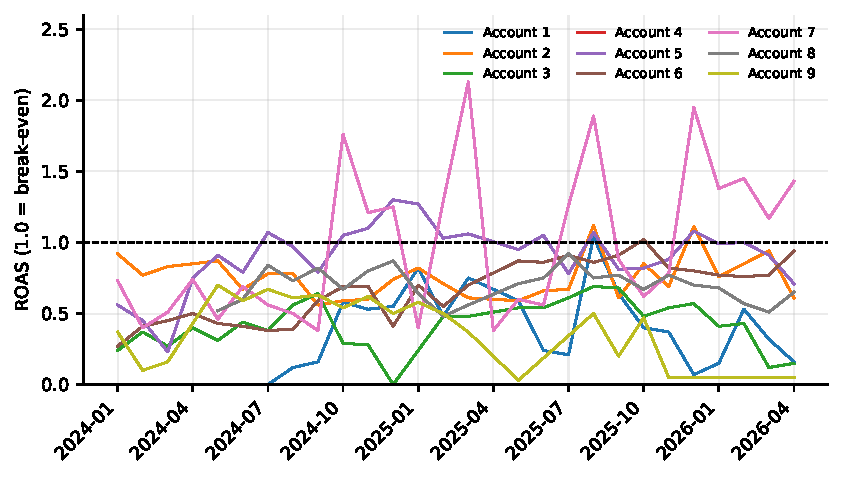
\includegraphics[width=0.92\linewidth]{fig/p2_roas.pdf}\caption{Monthly ROAS of the nine anonymised accounts since 2024; the dashed line is break-even.}\label{fig:roas}\end{figure}

\begin{figure}[H]\centering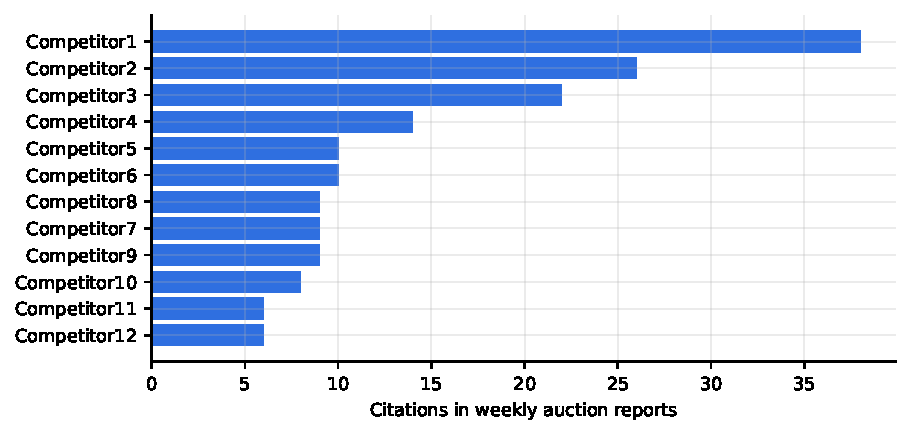
\includegraphics[width=0.8\linewidth]{fig/p2_comp.pdf}\caption{Competitors most often cited in weekly auction reports (anonymised labels).}\label{fig:comp}\end{figure}

\begin{figure}[H]\centering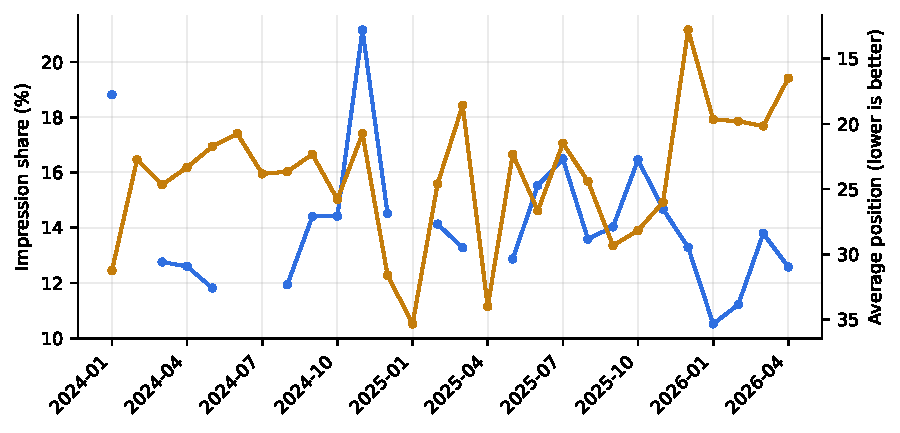
\includegraphics[width=0.8\linewidth]{fig/p2_is.pdf}\caption{Average impression share and position across accounts.}\label{fig:is}\end{figure}


\section{Diagnosis}
The worked example uses spend of 20,000\,\texteuro{} per month, ROAS 90\%, CPC 0.95\,\texteuro{}, conversion 9\% and impression share 15\%. These imply an EPL of 9.50\,\texteuro{}, a CPL of 10.56\,\texteuro{} and a break-even CPC of 0.85\,\texteuro{}. The account loses 2,000\,\texteuro{} a month in media. Figure~\ref{fig:heat} maps ROAS for combinations of CPC and conversion around this point: the account becomes profitable if either CPC falls by about 10\% or conversion rises by about 10\%.
\begin{figure}[H]\centering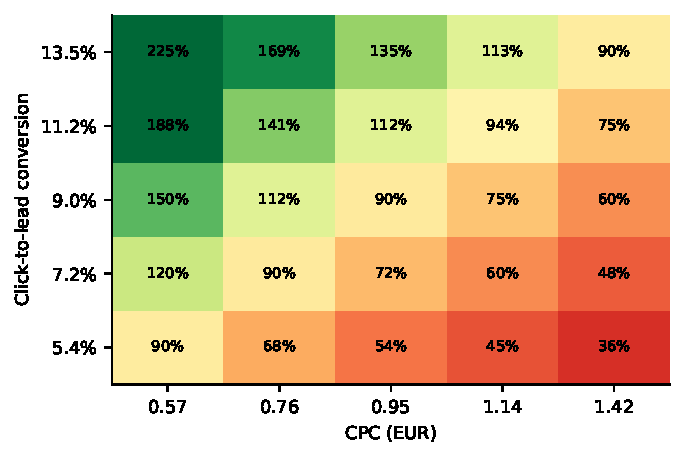
\includegraphics[width=0.62\linewidth]{fig/p2_heat.pdf}\caption{ROAS as a function of CPC and click-to-lead conversion for the worked example.}\label{fig:heat}\end{figure}
Figure~\ref{fig:tor} shows sensitivity to $\pm20\%$ changes. Conversion and EPL move profit by about 3,600\,\texteuro{} per 20\%, CPC by about 4,500\,\texteuro{}, and a 20\% rise in volume changes profit by -400\,\texteuro{}, because an account below break-even loses more as it scales.
\begin{figure}[H]\centering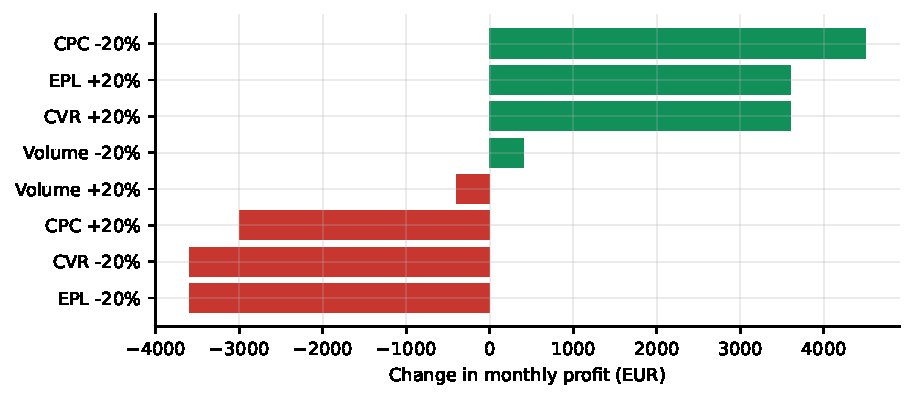
\includegraphics[width=0.8\linewidth]{fig/p2_tor.pdf}\caption{Change in monthly profit for $\pm20\%$ changes in each lever (worked example).}\label{fig:tor}\end{figure}

\subsection{Problem triage}
The tool accepts a stated problem and reorders actions. \emph{No traffic}: check impression share, bid and budget limits, and widen match types and signals. \emph{Traffic too expensive}: rewrite ads against competitors to lift quality, remove expensive keywords with low value, adjust schedules. \emph{Low conversion}: shorten the form, align landing pages with queries, and audit server-side tracking. \emph{Low quality}: separate low-quality demand, send values only for the partners that matter, and exclude existing users. \emph{ROAS falling}: audit tracking first, then review per-partner approval by campaign.

\subsection{Capacity}
If clicks scale with impression share, raising it from 15\% to a target $s$ gives $\text{clicks}\times s/15$. We assume CPC rises by $0.3\%$ for every 1\% of extra clicks. Table~\ref{tab:cap} gives the result for the example.
\begin{table}[H]\centering\small\caption{Click capacity in the worked example (baseline impression share 15\%).}\label{tab:cap}
\begin{tabular}{rrrr}\toprule Target share (\%) & Clicks & Extra clicks & CPC increase\\\midrule
15 & 21,053 & 0 & 0\%\\
25 & 35,088 & 14,035 & 20\%\\
35 & 49,123 & 28,070 & 40\%\\
45 & 63,158 & 42,105 & 60\%\\
60 & 84,211 & 63,158 & 90\%\\
\bottomrule\end{tabular}\end{table}

\section{Action catalogue and uplift}
Table~\ref{tab:acts} lists 15 actions with the relative change they induce in CPC, conversion, EPL and volume, as low-to-high ranges in percent, an effort score (1 easy, 3 hard), and the resulting monthly profit change in euros for the worked example (low / mid / high). The ranges are our hypotheses informed by the principles above.
\begin{table}[H]\centering\scriptsize\caption{Action catalogue (changes in percent; profit impact in euros per month).}\label{tab:acts}
\begin{tabular}{p{5.6cm}rrrrrr}\toprule Action & CPC & Conv. & EPL & Vol. & Effort & Impact (lo/mid/hi)\\\midrule
Per-campaign landing page and pingtree & -- & +8 to +20 & +3 to +8 & -- & 3 & 2,023 / 3,649 / 5,328\\
Audit server-side tracking by click ID and value feedback & -- & +5 to +20 & +2 to +6 & -- & 2 & 1,278 / 3,060 / 4,896\\
Rewrite ads with messages competitors use and you do not & -15 to -6 & +2 to +6 & -- & -- & 1 & 1,532 / 2,916 / 4,447\\
Add negative keywords from per-partner conversion value, not on day one & -12 to -5 & -- & +3 to +8 & -- & 2 & 1,516 / 2,754 / 4,091\\
Separate low-quality keywords into own campaigns and landing pages & -8 to -3 & -- & +4 to +10 & -- & 2 & 1,299 / 2,381 / 3,522\\
Exclude existing database users through an API & -3 to +0 & -- & +5 to +12 & -- & 2 & 900 / 1,827 / 2,784\\
Shorten the form and track step-level events & -- & +5 to +15 & -- & -- & 2 & 900 / 1,800 / 2,700\\
Reorder the pingtree by EPL and add partners & -- & -- & +5 to +15 & -- & 2 & 900 / 1,800 / 2,700\\
Send a CPL signal valued close to EPL on first-call acceptance & -- & +5 to +15 & -- & +8 to +20 & 2 & 812 / 1,772 / 2,840\\
Adjust schedules, devices and geographies with poor returns & -10 to -4 & -- & -- & -- & 1 & 750 / 1,355 / 2,000\\
Daily review, weekly optimisation and a change log & -5 to -2 & +2 to +5 & -- & -- & 1 & 735 / 1,306 / 1,895\\
Replace platform remarketing with an email and SMS flow & -- & -- & +4 to +10 & +0 to +5 & 2 & 720 / 1,242 / 1,790\\
Uncapped branded and competitor campaigns & -6 to -2 & -- & -- & +5 to +15 & 1 & 286 / 625 / 1,021\\
Allocate about 20\% to PMax and Demand Gen with proven creatives & -5 to +5 & -- & -- & +10 to +30 & 3 & -1,143 / -400 / 632\\
Test phrase and broad match with target CPA, about 500 EUR/day for new campaigns & +3 to +8 & -- & -- & +20 to +60 & 2 & -2,000 / -2,114 / -2,039\\
\bottomrule\end{tabular}\end{table}
\begin{figure}[H]\centering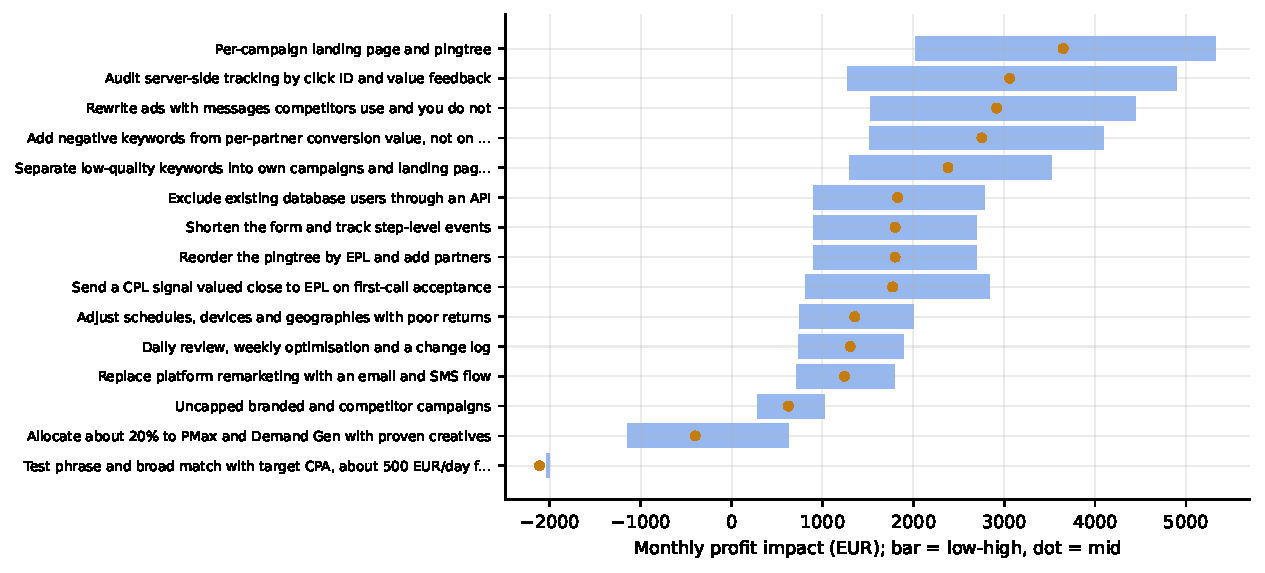
\includegraphics[width=0.95\linewidth]{fig/p2_actions.pdf}\caption{Estimated monthly profit impact of each action in the worked example.}\label{fig:act}\end{figure}

A plan of five actions (first-call CPL signal, excluding existing users, separate low-quality campaigns, value-based negative keywords and per-campaign landing pages) lifts ROAS to 115\%, 142\% and 173\% in the low, mid and high scenarios, and monthly profit from -2,000\,\texteuro{} to a steady state between 3,270\,\texteuro{} and 16,694\,\texteuro{}. With a three-month linear ramp, extra profit over six months is 26,351\,\texteuro{}, 55,724\,\texteuro{} and 93,472\,\texteuro{} (Figure~\ref{fig:proj}).
\begin{figure}[H]\centering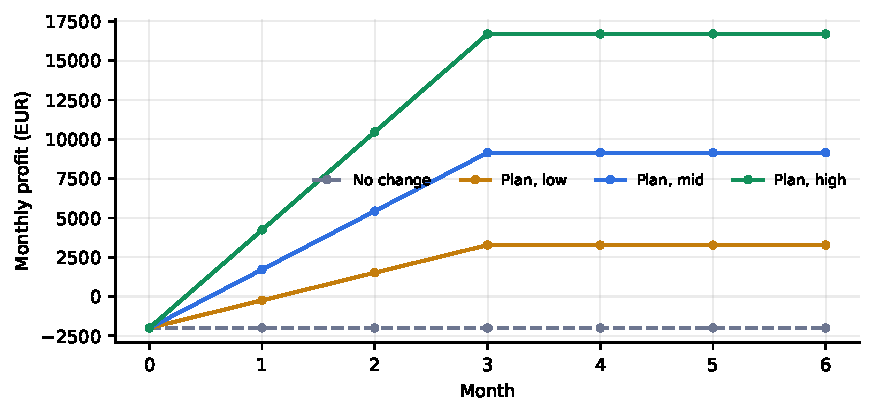
\includegraphics[width=0.8\linewidth]{fig/p2_proj.pdf}\caption{Monthly profit with no change and with the five-action plan.}\label{fig:proj}\end{figure}


\section{Ad-copy comparison}
Search ads are compared by message coverage. Each line of ad copy is tagged for nine claims: speed, amount, no fees, fully online, trust, flexibility, rate disclosure, call to action and urgency. The tool reports the share of lines that contain each claim for the advertiser and for pasted competitor copy, and lists claims that rivals use and the advertiser does not. It does not retrieve ads; the user pastes text from public ad libraries. Advertisers must still follow platform rules for financial services and local rate-disclosure requirements.

\section{Limitations}
(i) Uplift ranges are assumptions; they should be replaced by test results as soon as they exist. (ii) The tool analyses one account at a time and does not model cross-campaign cannibalisation. (iii) Reference-portfolio data are partial and anonymised, and conversion and CPC in the tool default to market-level guesses. (iv) Profit excludes staff, tooling and partner costs. (v) Impression share is a platform-reported number whose definition changes by campaign type.

\section{Conclusion}
Expressing an account as $\mathrm{ROAS}=ve/c$ makes diagnosis and prioritisation concrete: every action is a change in one of four numbers with a testable range. The next step is to run the highest-ranked actions as controlled tests and replace the hypothesised ranges with measured ones.

\begin{thebibliography}{9}
\bibitem{varian} H.~R. Varian. Position auctions. \emph{International Journal of Industrial Organization}, 25(6):1163--1178, 2007.
\bibitem{eos} B.~Edelman, M.~Ostrovsky, M.~Schwarz. Internet advertising and the generalized second-price auction. \emph{American Economic Review}, 97(1):242--259, 2007.
\end{thebibliography}
\end{document}
